
\begin{question}
In a very large population, 76.8\% are happy. When a random sample of
size 1600 is taken, what is the chance that the sample proportion of
happy individuals is beyond \(\pm\) 0.8 percentage points from 76.8\%?
\end{question}

\begin{solution}
Determine the standard error.
\[SE = \sqrt{\frac{p(1-p)}{n}} = \sqrt{\frac{0.768(1-0.768)}{1600}} = 0.011 \]
Determine the upper and lower bounds on \(\hat{p}\).
\[\hat{p}_{\text{lower}} = 0.768-0.008 = 0.76 \]
\[\hat{p}_{\text{upper}} = 0.768+0.008 = 0.776 \] Determine the \(z\)
scores. For simplicity, we ignore the continuity correction.
\[z_{\text{lower}} = \frac{\hat{p}_{\text{lower}}-p}{SE} = \frac{0.76-0.768}{0.011} = 
\frac{-0.008}{0.011} = -0.73 \]
\[z_{\text{upper}} = \frac{\hat{p}_{\text{upper}}-p}{SE} = \frac{0.776-0.768}{0.011} = \frac{0.008}{0.011} = 0.73 \]
We are looking for a two-tail area (``beyond \(\pm\) 0.8 percentage
points from 76.8\%'').

\begin{figure}[htbp]
\centering
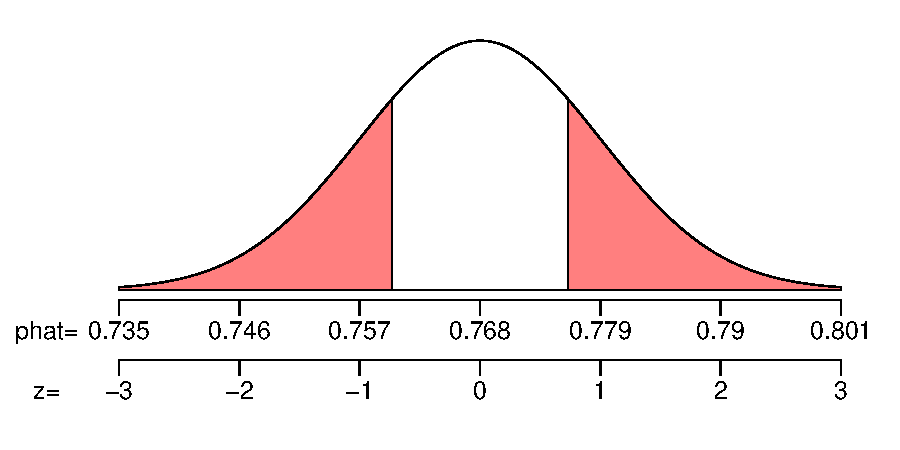
\includegraphics{phat_sampling_outer-1.pdf}
\caption{}
\end{figure}

To determine that central area, we use the z table.
\[\text{Pr}\left(|\hat{P}-0.768| > 0.008\right) ~~=~~ \text{Pr}\left(|Z| > 0.73\right) ~~=~~ 2\cdot\Phi(-0.73) ~~=~~ 0.4654 \]
Thus, we conclude there is a 46.5\% chance that the sample proportion is
beyond \(\pm\) 0.8 percentage points from 76.8\%.
\end{solution}

